\documentclass{article}
\usepackage{amsmath,ifthen,amsthm,amssymb,enumerate}
\usepackage[margin=1in]{geometry}
\usepackage[colorlinks=true,linkcolor=blue]{hyperref}
\usepackage{tikz,pgfplots}
\usepackage{tbil-de}
\usetikzlibrary{external}
\tikzexternalize 
\tikzset{%
  external/system call={pdflatex \tikzexternalcheckshellescape --halt-on-error --interaction=batchmode --output-directory=./aux --jobname "\image" "\texsource"},
  /pgf/images/include external/.code={%
    \includegraphics{aux/#1}%
  },
}



\newenvironment{problem}[1]
{
	\textbf{#1.}
	\ignorespaces
}{
\vspace{0.2in}
}

\newenvironment{solution}
{
	\textit{Solution.}
	\ignorespaces
}{
	\qed

	\vspace{1em}
}

\newcommand{\startModule}[1]
{
	\section*{Module #1}
	\addcontentsline{toc}{section}{Module #1}
}
\newcommand{\startStandard}[1]
{
	\subsection*{Standard #1}
	\addcontentsline{toc}{subsection}{Standard #1}
}

\begin{document}
\begin{flushleft}

\startModule{C}
\startStandard{C1}
\begin{problem}{C1}
Sketch a solution curve through each point marked in the slope field.

\begin{center}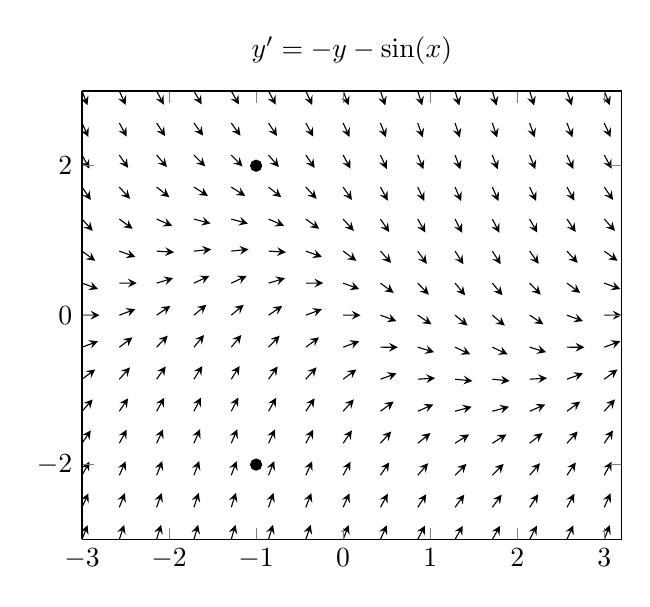
\begin{tikzpicture}
    \begin{axis}[
        title={\(y' = -y - \sin(x)\)},
        domain=-3:3,
        view={0}{90},
        axis background/.style={fill=white},
    ]
        \addplot3[black,
            quiver={
             u={1/(sqrt(1 + (-y - sin(60*x))^2)},
             v={(-y - sin(60*x))/(sqrt(1 + (-y - sin(60*x))^2)},
             scale arrows=0.2,
            },
            -stealth,samples=15]
                {exp(-x) - 1/2*sin(x) - 1/2*cos(x)};
        %KAWWWWWWW
        % Here be some points added to the swoopy loop vector fieldamagigs
        \addplot[mark=*] coordinates {(-1,2)}; % Obvious ordered pair for lococation
        \addplot[mark=*] coordinates {(-1,-2)};
    \end{axis}
\end{tikzpicture}\end{center}
\end{problem}

\begin{problem}{C1}
Sketch a solution curve through each point marked in the slope field.

\begin{center}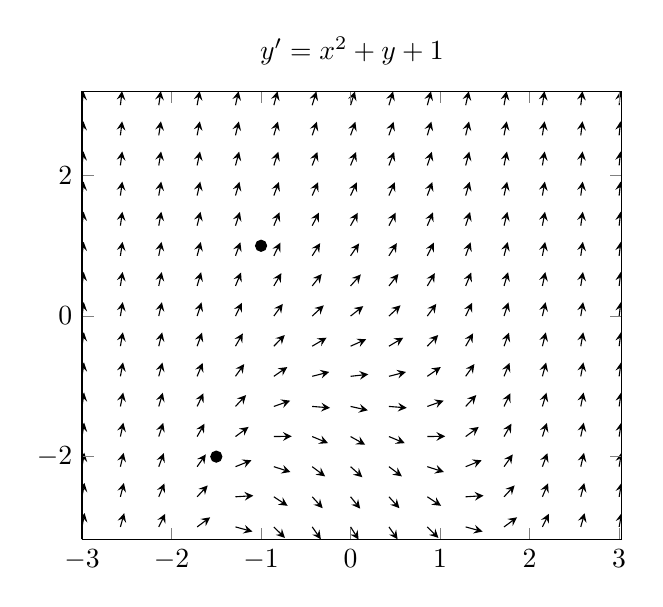
\begin{tikzpicture}
    \begin{axis}[
        title={\(y' = x^2 + y+1\)},
        domain=-3:3,
        view={0}{90},
        axis background/.style={fill=white},
    ]
        \addplot3[black,
            quiver={
             u={1/sqrt(1 + (x^2+y+1)^2)},
             v={(x^2 + y+1)/sqrt(1 + (x^2+y+1)^2)},
             scale arrows=0.2,
            },
            -stealth,samples=15]
                {exp(x) - x - 1};
        %KAWWWWWWW
        % Here be some points added to the swoopy loop vector fieldamagigs
        \addplot[mark=*] coordinates {(-1,1)}; % Obvious ordered pair for lococation
        \addplot[mark=*] coordinates {(-1.5,-2)};
    \end{axis}
\end{tikzpicture}\end{center}
\end{problem}

\begin{problem}{C1}
Sketch a solution curve through each point marked in the slope field.

\begin{center}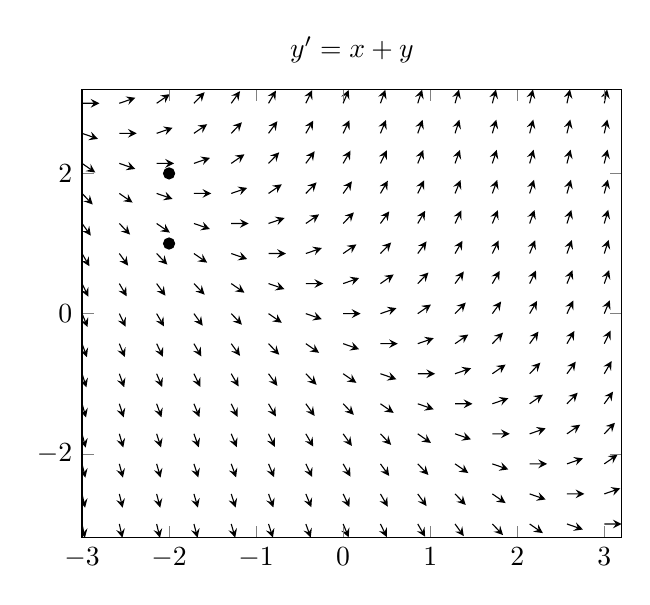
\begin{tikzpicture}
    \begin{axis}[
        title={\(y' = x + y\)},
        domain=-3:3,
        view={0}{90},
        axis background/.style={fill=white},
    ]
        \addplot3[black,
            quiver={
             u={1/sqrt(1 + (x+y)^2)},
             v={(x + y)/sqrt(1 + (x+y)^2)},
             scale arrows=0.2,
            },
            -stealth,samples=15]
                {exp(x) - x - 1};
        %KAWWWWWWW
        % Here be some points added to the swoopy loop vector fieldamagigs
        \addplot[mark=*] coordinates {(-2,1)}; % Obvious ordered pair for lococation
        \addplot[mark=*] coordinates {(-2,2)};
    \end{axis}
\end{tikzpicture}\end{center}
\end{problem}

\begin{problem}{C1}
Sketch a solution curve through each point marked in the slope field.

\begin{center}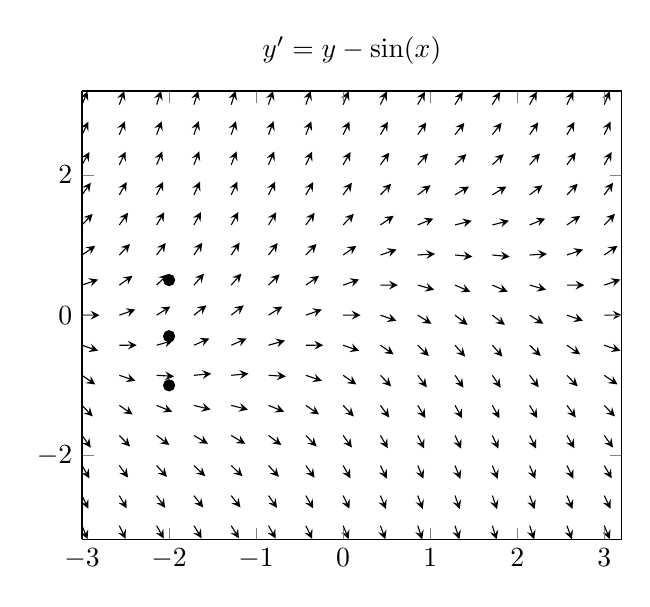
\begin{tikzpicture}
    \begin{axis}[
        title={\(y' = y - \sin(x)\)},
        domain=-3:3,
        view={0}{90},
        axis background/.style={fill=white},
    ]
        \addplot3[black,
            quiver={
             u={1/sqrt(1 + (y-sin(60*x))^2)},
             v={(y - sin(60*x))/sqrt(1 + (y-sin(60*x))^2)},
             scale arrows=0.2,
            },
            -stealth,samples=15]
                {exp(x) + 1/2*sin(x) + 1/2*cos(x)};
        %KAWWWWWWW
        % Here be some points added to the swoopy loop vector fieldamagigs
        \addplot[mark=*] coordinates {(-2,-1)}; % Obvious ordered pair for lococation
        \addplot[mark=*] coordinates {(-2,-.3)};
        \addplot[mark=*] coordinates {(-2,.5)};
    \end{axis}
\end{tikzpicture}\end{center}
\end{problem}

\begin{problem}{C1}
Sketch a solution curve through each point marked in the slope field.

\begin{center}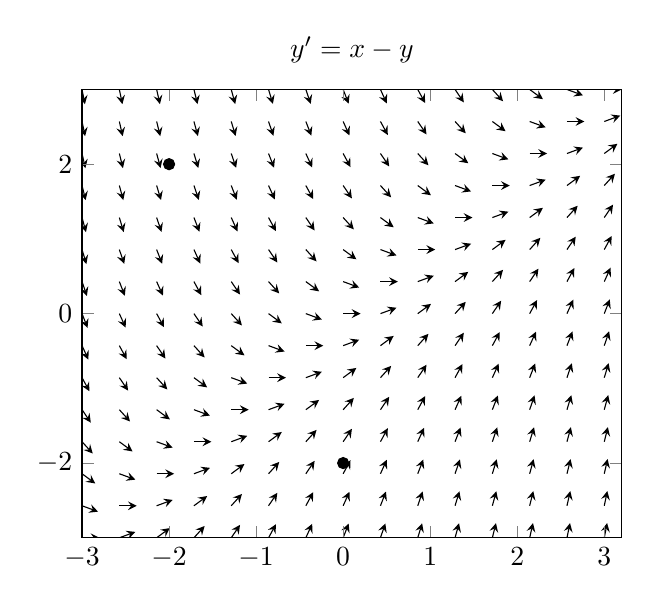
\begin{tikzpicture}
    \begin{axis}[
        title={\(y' = x - y\)},
        domain=-3:3,
        view={0}{90},
        axis background/.style={fill=white},
    ]
        \addplot3[black,
            quiver={
             u={1/sqrt(1 + (x - y)^2)},
             v={(x - y)/sqrt(1 + (x - y)^2)},
             scale arrows=0.2,
            },
            -stealth,samples=15]
                {exp(-x) + x - 1};
        \addplot[mark=*] coordinates {(-2,2)};
        \addplot[mark=*] coordinates {(0,-2)};
    \end{axis}
\end{tikzpicture}\end{center}
\end{problem}

\begin{problem}{C1}
Sketch a solution curve through each point marked in the slope field.

\begin{center}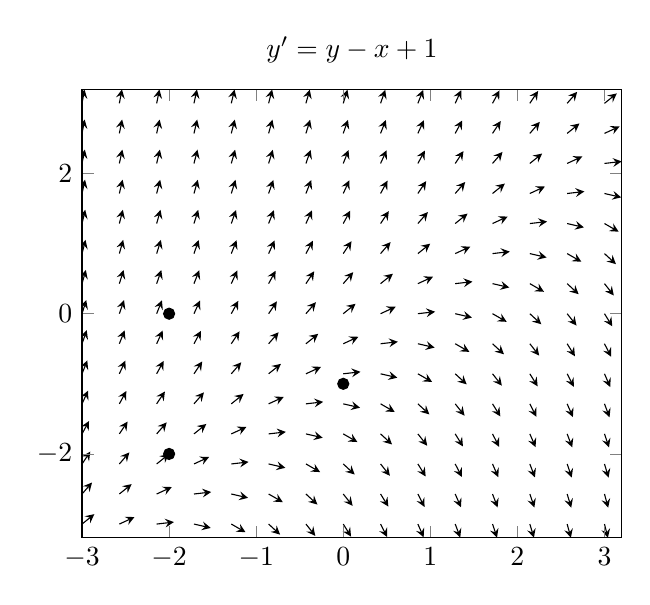
\begin{tikzpicture}
    \begin{axis}[
        title={\(y' = y - x + 1\)},
        domain=-3:3,
        view={0}{90},
        axis background/.style={fill=white},
    ]
        \addplot3[black,
            quiver={
             u={1/sqrt(1 + (y - x + 1)^2)},
             v={(y - x + 1)/sqrt(1 + (y - x + 1)^2)},
             scale arrows=0.2,
            },
            -stealth,samples=15]
                {exp(x) + x};
        \addplot[mark=*] coordinates {(-2,-2)};
        \addplot[mark=*] coordinates {(-2,0)};
        \addplot[mark=*] coordinates {(0,-1)};
    \end{axis}
\end{tikzpicture}\end{center}
\end{problem}

\begin{problem}{C1}
Sketch a solution curve through each point marked in the slope field.

\begin{center}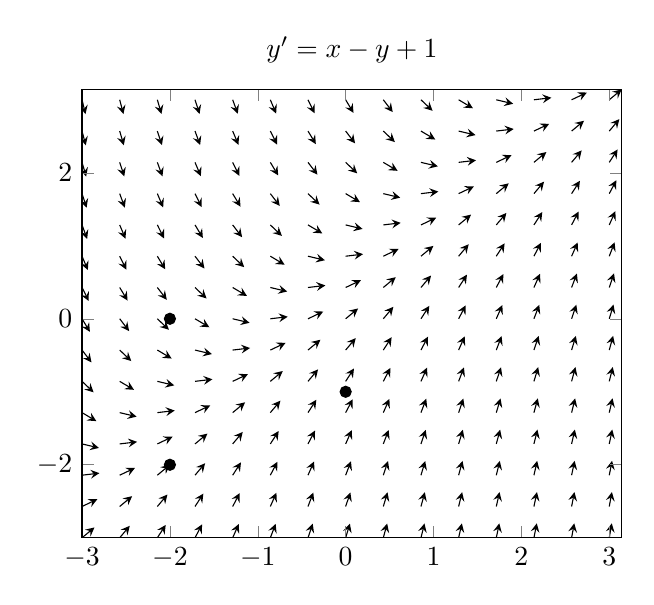
\begin{tikzpicture}
    \begin{axis}[
        title={\(y' = x - y + 1\)},
        domain=-3:3,
        view={0}{90},
        axis background/.style={fill=white},
    ]
        \addplot3[black,
            quiver={
             u={1/sqrt(1 + (x - y + 1)^2)},
             v={(x - y + 1)/sqrt(1 + (x - y + 1)^2)},
             scale arrows=0.2,
            },
            -stealth,samples=15]
                {exp(-x) + x};
        \addplot[mark=*] coordinates {(-2,-2)};
        \addplot[mark=*] coordinates {(-2,0)};
        \addplot[mark=*] coordinates {(0,-1)};
    \end{axis}
\end{tikzpicture}\end{center}
\end{problem}

\begin{problem}{C1}
Sketch a solution curve through each point marked in the slope field.

\begin{center}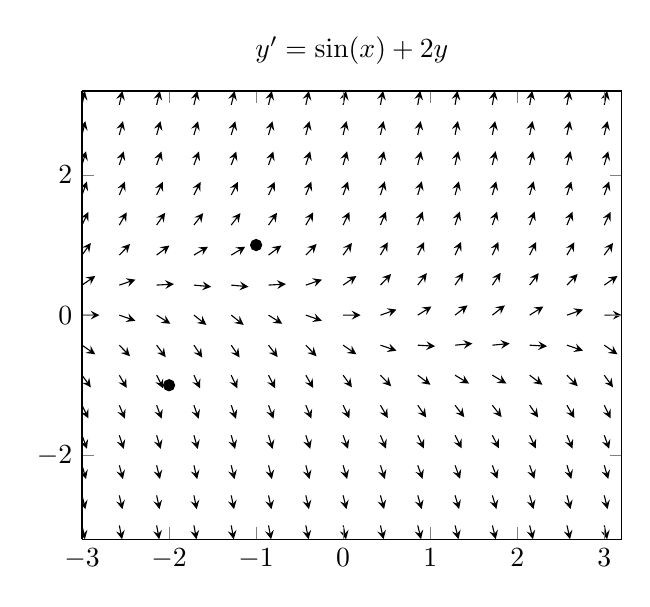
\begin{tikzpicture}
    \begin{axis}[
        title={\(y' = \sin(x) + 2y\)},
        domain=-3:3,
        view={0}{90},
        axis background/.style={fill=white},
    ]
        \addplot3[black,
            quiver={
             u={1/sqrt(1 + (sin(60*x) + 2*y)^2)},
             v={(sin(60*x) +2*y)/sqrt(1 + (sin(60*x) + 2*y)^2)},
             scale arrows=0.2,
            },
            -stealth,samples=15]
                {x};
        \addplot[mark=*] coordinates {(-1,1)};
        \addplot[mark=*] coordinates {(-2,-1)};
    \end{axis}
\end{tikzpicture}\end{center}
\end{problem}

\begin{problem}{C1}
Sketch a solution curve through each point marked in the slope field.

\begin{center}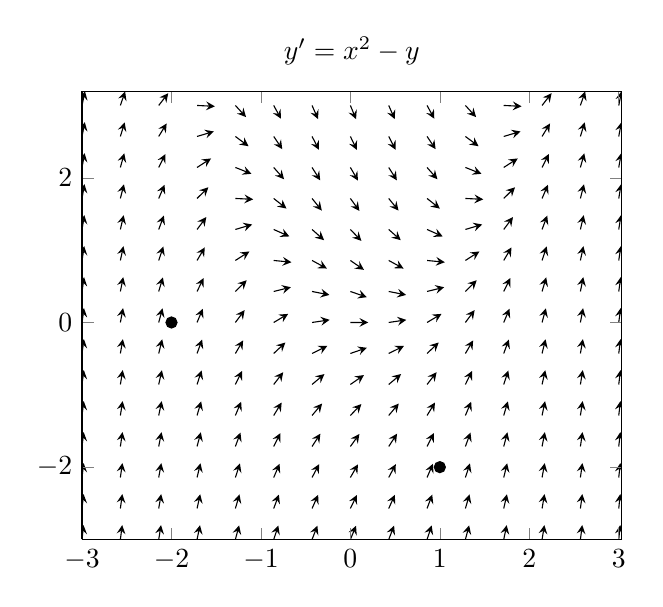
\begin{tikzpicture}
    \begin{axis}[
        title={\(y' = x^2 - y\)},
        domain=-3:3,
        view={0}{90},
        axis background/.style={fill=white},
    ]
        \addplot3[black,
            quiver={
             u={1/sqrt(1 + (x^2 - y)^2)},
             v={(x^2 - y)/sqrt(1 + (x^2 - y)^2)},
             scale arrows=0.2,
            },
            -stealth,samples=15]
                {x};
        \addplot[mark=*] coordinates {(-2,0)};
        \addplot[mark=*] coordinates {(1,-2)};
    \end{axis}
\end{tikzpicture}\end{center}
\end{problem}

 \newpage
\begin{problem}{C2}
A water droplet with a radius of \(100\ {\rm \mu m}\) has a mass of about \(4 \times 10^{-12} {\rm kg}\) and a terminal velocity of \(27\ {\rm \frac{cm}{s}}\).  Such a droplet is dropped from rest.  
\begin{enumerate}[(a)]
\item Write down an Initial Value Problem (IVP) modelling the velocity.
\item What is its velocity after \(0.01\ {\rm s}\)?
\end{enumerate}
\end{problem}

\begin{problem}{C2}
A water droplet with a radius of \(50\ {\rm \mu m}\) has a mass of about \(5 \times 10^{-13} {\rm kg}\) and a terminal velocity of \(3.5\ {\rm \frac{cm}{s}}\).  Such a droplet is dropped from rest.  
\begin{enumerate}[(a)]
\item Write down an Initial Value Problem (IVP) modelling the velocity.
\item What is its velocity after \(0.01\ {\rm s}\)?
\end{enumerate}
\end{problem}

\begin{problem}{C2}
A water droplet with a radius of \(10\ {\rm \mu m}\) has a mass of about \(4 \times 10^{-15} {\rm kg}\) and a terminal velocity of \(270 \ {\rm \frac{\mu m}{s}}\).  Such a droplet is dropped from rest.  
\begin{enumerate}[(a)]
\item Write down an Initial Value Problem (IVP) modelling the velocity.
\item What is its velocity after \(0.001\ {\rm s}\)?
\end{enumerate}
\end{problem}

\begin{problem}{C2}
A water droplet with a radius of \(5\ {\rm \mu m}\) has a mass of about \(5 \times 10^{-16} {\rm kg}\) and a terminal velocity of \(35 \ {\rm \frac{\mu m}{s}}\).  Such a droplet is dropped from rest.  
\begin{enumerate}[(a)]
\item Write down an Initial Value Problem (IVP) modelling the velocity.
\item What is its velocity after \(0.001\ {\rm s}\)?
\end{enumerate}
\end{problem}

\begin{problem}{C2}
A single grain of corn pollen with a radius of \(50\ {\rm \mu m}\) and a mass of about \(5 \times 10^{-13} {\rm kg}\) has a terminal velocity of \(27\ {\rm \frac{cm}{s}}\).  Such a pollen grain is dropped from rest.  
\begin{enumerate}[(a)]
\item Write down an Initial Value Problem (IVP) modelling the velocity.
\item What is its velocity after \(0.01\ {\rm s}\)?
\end{enumerate}
\end{problem}

\begin{problem}{C2}
A single grain of spruce pollen with a radius of \(25\ {\rm \mu m}\) and a mass of about \(6 \times 10^{-14} {\rm kg}\) has a terminal velocity of \(3\ {\rm \frac{cm}{s}}\).  Such a pollen grain is dropped from rest.  
\begin{enumerate}[(a)]
\item Write down an Initial Value Problem (IVP) modelling the velocity.
\item What is its velocity after \(0.01\ {\rm s}\)?
\end{enumerate}
\end{problem}



 \newpage
\begin{problem}{C3}
Find the general solution to
\[
y'' + 2y' + y = 0.
\]
\end{problem}

\begin{problem}{C3}
Find the general solution to
\[
y'' + 2y' - 8y = 0.
\]
\end{problem}

\begin{problem}{C3}
Find the general solution to
\[
y'' + 4y' + 3y = 0.
\]
\end{problem}

\begin{problem}{C3}
Find the general solution to
\[
y'' + 2y' - 3y = 0.
\]
\end{problem}

\begin{problem}{C3}
Find the general solution to
\[
y'' - 2y' - 3y = 0.
\]
\end{problem}

\begin{problem}{C3}
Find the general solution to
\[
y'' + 4y' + 4y = 0.
\]

\end{problem}

\begin{problem}{C3}
Find the general solution to
\[
y'' - 4y' + 4y = 0.
\]
\end{problem}

\begin{problem}{C3}
Find the general solution to
\[
y'' + 5y' + 6y = 0.
\]
\end{problem}


%Add more complex roots
\begin{problem}{C3}
Find the general solution to
\[
y'' - 2y' + 2y = 0.
\]
\end{problem}

\begin{problem}{C3}
Find the general solution to
\[
y'' + 2y' + 2y = 0.
\]
\end{problem}
 \newpage
\begin{problem}{C4}
Find a general solution to the given equation.
\[
y'' + 2y' + y = 3x + 4
\]
\end{problem}


\begin{problem}{C4}
Find a general solution to the given equation.
\[
y'' + 4y' + 3y = 2\sin(3x)
\]
\end{problem}


\begin{problem}{C4}
Find a general solution to the given equation.
\[
y'' - 2y' - 3y = 1 + xe^x
\]
\end{problem}


\begin{problem}{C4}
Find a general solution to the given equation.
\[
y'' - 4y' + 4y = e^{2x}
\]
\end{problem}

\begin{problem}{C4}
Find a general solution to the given equation.
\[
y'' + 4y' + 4y = e^{2x}
\]
\end{problem}




\begin{problem}{C4}
Find a general solution to the given equation.
\[
y'' + 4y = \cos(2x)
\]
\end{problem}

\begin{problem}{C4}
Find a general solution to the given equation.
\[
y'' - 4y = \cos(2x)
\]
\end{problem}


\begin{problem}{C4}
Find a general solution to the given equation.
\[
y'' + 9y = \sin(3x)
\]
\end{problem}

\begin{problem}{C4}
Find a general solution to the given equation.
\[
y'' - 9y = \sin(3x)
\]
\end{problem}


\begin{problem}{C4}
Find a general solution to the given equation.
\[
y'' - 2y' + 2y = \sin(x)
\]
\end{problem}


\begin{problem}{C4}
Find a general solution to the given equation.
\[
y'' - 2y' + 5y = 2x + 1
\]
\end{problem}



 \newpage
\begin{problem}{C5}
Find a general solution to the given equation.
\[
y'' + 3y' + 2y = 6 e^x 
\]
\end{problem}

\begin{problem}{C5}
Find a general solution to the given equation.
\[
y'' + 3y' + 2y = 100 e^{3x} 
\]
\end{problem}


\begin{problem}{C5}
Find a general solution to the given equation.
\[
y'' + 4y' + 3y = 15 e^{2x}
\]
\end{problem}

\begin{problem}{C5}
Find a general solution to the given equation.
\[
y'' + 4y' + 3y = 16 e^{x}
\]
\end{problem}


\begin{problem}{C5}
Find a general solution to the given equation.
\[
y'' - 2y' - 3y = 24 e^{5x}
\]
\end{problem}


\begin{problem}{C5}
Find a general solution to the given equation.
\[
y'' - 4y' + 4y = 16 e^{-2x}
\]
\end{problem}

\begin{problem}{C5}
Find a general solution to the given equation.
\[
y'' + 4y' + 4y = 16 e^{2x}
\]
\end{problem}

\begin{problem}{C5}
Find a general solution to the given equation.
\[
y'' + 5y' + 6y = 24 e^{x}
\]
\end{problem}


\begin{problem}{C5}
Find a general solution to the given equation.
\[
y'' + 5y' + 6y = 24 e^{-x}
\]
\end{problem}

\begin{problem}{C5}
Find a general solution to the given equation.
\[
y'' + 7y' + 12y = 60 e^{x}
\]
\end{problem}

\begin{problem}{C5}
Find a general solution to the given equation.
\[
y'' + 7y' + 12y = 60 e^{-x}
\]
\end{problem}
 \newpage
\begin{problem}{C6}
Consider the following scenario:
A \(1 {\rm kg}\) mass is suspended by a spring (with spring constant \(4 {\rm kg /s^2}\)).  The mass is pulled down \(1 {\rm m}\) from its equillibrium position and released from rest.  
\begin{enumerate}[(a)]
\item Write down an IVP modelling the position of the mass.
\item How long does it take for the mass to return to its equillibrium point?
\end{enumerate}
\end{problem}

\begin{problem}{C6}
Consider the following scenario:
A \(1 {\rm kg}\) mass is suspended by a spring (with spring constant \(4 {\rm kg /s^2}\)).  The mass is pushed up \(0.5 {\rm m}\) from its equillibrium position and released from rest.  
\begin{enumerate}[(a)]
\item Write down an IVP modelling the position of the mass.
\item How long does it take for the mass to return to its equillibrium point?
\end{enumerate}
\end{problem}

\begin{problem}{C6}
Consider the following scenario:
A \(4 {\rm kg}\) mass is suspended by a spring (with spring constant \(1 {\rm kg /s^2}\)).  The mass is pulled down \(1 {\rm m}\) from its equillibrium position and released from rest.  
\begin{enumerate}[(a)]
\item Write down an IVP modelling the position of the mass.
\item Where is the mass after \(3 {\rm s}\)?
\end{enumerate}
\end{problem}

\begin{problem}{C6}
Consider the following scenario:
A \(4 {\rm kg}\) mass is suspended by a spring (with spring constant \(1 {\rm kg /s^2}\)).  The mass is pushed up \(0.5 {\rm m}\) from its equillibrium position and released from rest.  
\begin{enumerate}[(a)]
\item Write down an IVP modelling the position of the mass.
\item Where is the mass after \(2 {\rm s}\)?
\end{enumerate}
\end{problem}

\begin{problem}{C6}
Consider the following scenario:
A \(2 {\rm kg}\) mass is suspended by a spring (with spring constant \(4 {\rm kg /s^2}\)).  A linear damper is attached to the system (with constant \(6 {\rm kg/s}\).  The mass is pulled down \(1 {\rm m}\) from its equillibrium position and released from rest.  
\begin{enumerate}[(a)]
\item Write down an IVP modelling the position of the mass.
\item Where is the mass after \(2 {\rm s}\)?
\end{enumerate}
\end{problem}

\begin{problem}{C6}
Consider the following scenario:
A \(2 {\rm kg}\) mass is suspended by a spring (with spring constant \(4 {\rm kg /s^2}\)).  A linear damper is attached to the system (with constant \(1 {\rm kg/s}\).  The mass is pulled down \(1 {\rm m}\) from its equillibrium position and released from rest.  
\begin{enumerate}[(a)]
\item Write down an IVP modelling the position of the mass.
\item Where is the mass after \(2 {\rm s}\)?
\end{enumerate}
\end{problem}





\begin{problem}{C6}
Consider the following scenario:
A \(2 {\rm kg}\) mass is suspended by a spring (with spring constant \(4 {\rm kg /s^2}\)).  A linear damper is attached to the system (with constant \(6 {\rm kg/s}\).  An external force is applied, modelled by the function \(F(t)=200e^{-5t}\).  The mass is pulled down \(1 {\rm m}\) from its equillibrium position and released from rest.  
\begin{enumerate}[(a)]
\item Write down an IVP modelling the position of the mass.
\item Where is the mass after \(2 {\rm s}\)?
\end{enumerate}
\end{problem}

\begin{problem}{C6}
Consider the following scenario:
A \(2 {\rm kg}\) mass is suspended by a spring (with spring constant \(4 {\rm kg /s^2}\)).  A linear damper is attached to the system (with constant \(6 {\rm kg/s}\).  An external force is applied, modelled by the function \(F(t)=200e^{-5t}\).  The mass is pulled down \(1 {\rm m}\) from its equillibrium position and released from rest.  
\begin{enumerate}[(a)]
\item Write down an IVP modelling the position of the mass.
\item Where is the mass after \(2 {\rm s}\)?
\end{enumerate}
\end{problem}
 \newpage

\startModule{F}
\startStandard{F1}
\input{modules/2-F/exercises/F1.tex} \newpage
\begin{problem}{F2}
Find the general solution to \(\frac{dy}{dx} + 3xy = 0\).
\end{problem}

\begin{problem}{F2}
Find the general solution to \(y' - y\sin(x)=0\).
\end{problem} 

\begin{problem}{F2}
Find the general solution to \(y' - y^2e^x=0\).
\end{problem} 

\begin{problem}{F2}
Find the general solution to \(y' = \frac{x+2}{y^2}\).
\end{problem}


\begin{problem}{F2}
Find the general solution to \(xy' = y\).
\end{problem}

\begin{problem}{F2}
Find the general solution to \(y\frac{dy}{dx} = y^2\cos(x)\).
\end{problem}

\begin{problem}{F2}
Find the general solution to \(xy^2\frac{dy}{dx} = 1\).
\end{problem}

\begin{problem}{F2}
Find the general solution to \(x\cos(y)y' = 1\).
\end{problem}
 \newpage
\begin{problem}{F3}
Find the general solution to \(xy' + 4y = 2x\).
\end{problem}

\begin{problem}{F3}
Find the general solution to \(xy' + 4y = \sqrt{x}\) (for \(x>0\)).
\end{problem}

\begin{problem}{F3}
Find the general solution to \(xy' + 2y = x^2\).
\end{problem}

\begin{problem}{F3}
Find the general solution to \(y' = 2 + x + 2y + xy\).
\end{problem}

\begin{problem}{F3}
Find the general solution to \(y' = 1 + 2x + y + 2xy\).
\end{problem}

 \newpage
\begin{problem}{F4}
Find the general solution to \(xy' + 4y = 2x\).
\end{problem}

\begin{problem}{F4}
Find the general solution to \(xy' + 4y = \sqrt{x}\) (for \(x>0\)).
\end{problem}

\begin{problem}{F4}
Find the general solution to \(xy' + 2y = x^2\).
\end{problem}

\begin{problem}{F4}
Find the general solution to \(y' = 1 + 2x + y + 2xy\).
\end{problem}

 \newpage
\begin{problem}{F5}
Find the general solution to \(xy' + 4y = 2x\).
\end{problem}

\begin{problem}{F5}
Find the general solution to \(xy' + 4y = \sqrt{x}\) (for \(x>0\)).
\end{problem}

\begin{problem}{F5}
Find the general solution to \(xy' + 2y = x^2\).
\end{problem}

\begin{problem}{F5}
Find the general solution to \(xy' + 2y = 4x^2-3x\).
\end{problem}

\begin{problem}{F5}
Find the general solution to \(xy' + 2y = x^2-3x\).
\end{problem}

\begin{problem}{F5}
Find the general solution to \(\cos(x) y' + \sin (x)y = x +\sin(x)\cos(x) \).
\end{problem}

\begin{problem}{F5}
Find the general solution to \(\cos(x) y' + \sin (x)y = x \cos^2(x) \).
\end{problem}

\begin{problem}{F5}
Find the general solution to \((x^2+1)y' - xy =1 \).
\end{problem}

\begin{problem}{F5}
Find the general solution to \((x^2+1)y' - xy =x+1 \).
\end{problem}
 \newpage
\input{modules/2-F/exercises/F6.tex} \newpage


\startModule{S}
\startStandard{S1}
\begin{problem}{S1}
Find the general solution of the system
\begin{align*}
x' & = x + y,\\
y' & = 4x + y.\\
\end{align*}
\end{problem}

\begin{problem}{S1}
Find the general solution of the system
\begin{align*}
x' & = x + 2y,\\
y' & = 3x + 2y.\\
\end{align*}
\end{problem}

\begin{problem}{S1}
Find the general solution of the system
\begin{align*}
x' & = 2x + y,\\
y' & = x + 2y.\\
\end{align*}
\end{problem}

\begin{problem}{S1}
Find the general solution of the system
\begin{align*}
x' & = 2x +  y,\\
y' & = 2x + 3y.\\
\end{align*}
\end{problem}

\begin{problem}{S1}
Find the general solution of the system
\begin{align*}
x' & = 3x + y,\\
y' & = x +  3y.\\
\end{align*}
\end{problem}

\begin{problem}{S1}
Find the general solution of the system
\begin{align*}
x' & = 3x + y,\\
y' & = 2x + 2y.\\
\end{align*}
\end{problem}

\begin{problem}{S1}
Find the general solution of the system
\begin{align*}
x' & = 4x + y,\\
y' & = 2x + 3y.\\
\end{align*}
\end{problem}

\begin{problem}{S1}
Find the general solution of the system
\begin{align*}
x' & = 4x + 3y,\\
y' & = x + 2y.\\
\end{align*}
\end{problem}

 \newpage
%\begin{problem}{S2}
\end{problem}

 \newpage
%\begin{problem}{S3}
\begin{minipage}[t]{0.8\linewidth}
Consider the dual mass-spring system at the right.  Both masses are \(1 {\rm kg}\).  The upper spring has a spring constant of \( 1 {\rm N/m}\) while the lower spring constant is \(6 {\rm N/m}\).  The lower mass is pulled down \(1 {\rm m}\) without disturbing the upper mass, and released from rest. 
\begin{enumerate}[(a)]
\item Write down an IVP modelling the motion of the two masses.
\item Where will the two masses be after \(2 {\rm s}\)?
\end{enumerate}
\end{minipage}
\hfill
\springdoublemassQuiz[0.7]
\hfill
\end{problem}

\begin{problem}{S3}
\begin{minipage}[t]{0.8\linewidth}
Consider the dual mass-spring system at the right.  Both masses are \(1 {\rm kg}\).  The upper spring has a spring constant of \( 1 {\rm N/m}\) while the lower spring constant is \(6 {\rm N/m}\).  The lower mass is pulled down \(0.5 {\rm m}\) without disturbing the upper mass, and released from rest. 
\begin{enumerate}[(a)]
\item Write down an IVP modelling the motion of the two masses.
\item Where will the two masses be after \(3 {\rm s}\)?
\end{enumerate}
\end{minipage}
\hfill
\springdoublemassQuiz[0.7]
\hfill
\end{problem}

\begin{problem}{S3}
\begin{minipage}[t]{0.8\linewidth}
Consider the dual mass-spring system at the right.  Both masses are \(1 {\rm kg}\).  The upper spring has a spring constant of \( 1 {\rm N/m}\) while the lower spring constant is \(6 {\rm N/m}\).  The upper mass is pushed up \(0.5 {\rm m}\) without disturbing the lower mass, and released from rest. 
\begin{enumerate}[(a)]
\item Write down an IVP modelling the motion of the two masses.
\item Where will the two masses be after \(4 {\rm s}\)?
\end{enumerate}
\end{minipage}
\hfill
\springdoublemassQuiz[0.7]
\hfill
\end{problem}

\begin{problem}{S3}
\begin{minipage}[t]{0.8\linewidth}
Consider the dual mass-spring system at the right.  Both masses are \(3 {\rm kg}\).  The upper spring has a spring constant of \( 8 {\rm N/m}\) while the lower spring constant is \(6 {\rm N/m}\).  The upper mass is pushed up \(0.5 {\rm m}\) without disturbing the lower mass, and released from rest. 
\begin{enumerate}[(a)]
\item Write down an IVP modelling the motion of the two masses.
\item Where will the two masses be after \(2 {\rm s}\)?
\end{enumerate}
\end{minipage}
\hfill
\springdoublemassQuiz[0.7]
\hfill
\end{problem}

\begin{problem}{S3}
\begin{minipage}[t]{0.8\linewidth}
Consider the dual mass-spring system at the right.  Both masses are \(3 {\rm kg}\).  The upper spring has a spring constant of \( 8 {\rm N/m}\) while the lower spring constant is \(6 {\rm N/m}\).  The lower mass is pulled down \(0.5 {\rm m}\) without disturbing the upper mass, and released from rest. 
\begin{enumerate}[(a)]
\item Write down an IVP modelling the motion of the two masses.
\item Where will the two masses be after \(2 {\rm s}\)?
\end{enumerate}
\end{minipage}
\hfill
\springdoublemassQuiz[0.7]
\hfill
\end{problem}

\begin{problem}{S3}
\begin{minipage}[t]{0.8\linewidth}
Consider the dual mass-spring system at the right.  The upper mass is \(2 {\rm kg}\) while the lower mass is \(1 {\rm kg}\).  The upper spring has a spring constant of \( 6 {\rm N/m}\) while the lower spring constant is \(4 {\rm N/m}\).  The lower mass is pulled down \(0.5 {\rm m}\) without disturbing the upper mass, and released from rest. 
\begin{enumerate}[(a)]
\item Write down an IVP modelling the motion of the two masses.
\item Where will the two masses be after \(3 {\rm s}\)?
\end{enumerate}
\end{minipage}
\hfill
\springdoublemassQuiz[0.7]
\hfill
\end{problem}

\begin{problem}{S3}
\begin{minipage}[t]{0.8\linewidth}
Consider the dual mass-spring system at the right.  The upper mass is \(2 {\rm kg}\) while the lower mass is \(1 {\rm kg}\).  The upper spring has a spring constant of \( 6 {\rm N/m}\) while the lower spring constant is \(4 {\rm N/m}\).  The lower mass is pulled down \(1 {\rm m}\) without disturbing the upper mass, and released from rest. 
\begin{enumerate}[(a)]
\item Write down an IVP modelling the motion of the two masses.
\item Where will the two masses be after \(2 {\rm s}\)?
\end{enumerate}
\end{minipage}
\hfill
\springdoublemassQuiz[0.7]
\hfill
\end{problem}

\begin{problem}{S3}
\begin{minipage}[t]{0.8\linewidth}
Consider the dual mass-spring system at the right.  The upper mass is \(1 {\rm kg}\) while the lower mass is \(2 {\rm kg}\).  The upper spring has a spring constant of \( 3 {\rm N/m}\) while the lower spring constant is \(4 {\rm N/m}\).  The lower mass is pulled down \(0.5 {\rm m}\) without disturbing the upper mass, and released from rest. 
\begin{enumerate}[(a)]
\item Write down an IVP modelling the motion of the two masses.
\item Where will the two masses be after \(3 {\rm s}\)?
\end{enumerate}
\end{minipage}
\hfill
\springdoublemassQuiz[0.7]
\hfill
\end{problem}

\begin{problem}{S3}
\begin{minipage}[t]{0.8\linewidth}
Consider the dual mass-spring system at the right.  The upper mass is \(1 {\rm kg}\) while the lower mass is \(2 {\rm kg}\).  The upper spring has a spring constant of \( 3 {\rm N/m}\) while the lower spring constant is \(4 {\rm N/m}\).  The lower mass is pulled down \(1 {\rm m}\) without disturbing the upper mass, and released from rest. 
\begin{enumerate}[(a)]
\item Write down an IVP modelling the motion of the two masses.
\item Where will the two masses be after \(2 {\rm s}\)?
\end{enumerate}
\end{minipage}
\hfill
\springdoublemassQuiz[0.7]
\hfill
\end{problem}
 \newpage



\startModule{N}
\startStandard{N1}
\begin{problem}{N1}
Determine whether existence of at least one solution of the given initial value problem
is guaranteed and, if so, whether uniqueness of that solution is guaranteed.
\[
y' = x^2y + xy^2; \,\,\,\,\,\,\,\,\,y(1) = 3
\]
\end{problem}

\begin{problem}{N1}
Determine whether existence of at least one solution of the given initial value problem
is guaranteed and, if so, whether uniqueness of that solution is guaranteed.
\[
y' = 2x^2 + xy + 3y^2;\,\,\,\,\,\,\,\,\,y(1) = -1
\]
\end{problem}

\begin{problem}{N1}
Determine whether existence of at least one solution of the given initial value problem
is guaranteed and, if so, whether uniqueness of that solution is guaranteed.
\[
y' = x + \ln(y);\,\,\,\,\,\,\,\,\,y(1) = 2
\]
\end{problem}

\begin{problem}{N1}
Determine whether existence of at least one solution of the given initial value problem
is guaranteed and, if so, whether uniqueness of that solution is guaranteed.
\[
y' = \sqrt{x+y};\,\,\,\,\,\,\,\,\,y(1) = 1
\]
\end{problem}

\begin{problem}{N1}
Determine whether existence of at least one solution of the given initial value problem
is guaranteed and, if so, whether uniqueness of that solution is guaranteed.
\[
y' = \sqrt[3]{x-y};\,\,\,\,\,\,\,\,\,y(2) = 2
\]
\end{problem}

\begin{problem}{N1}
Determine whether existence of at least one solution of the given initial value problem
is guaranteed and, if so, whether uniqueness of that solution is guaranteed.
\[
y' = \frac{y}{x};\,\,\,\,\,\,\,\,\,y(2) = 1
\]
\end{problem}

 \newpage


\begin{problem}{N2}
Consider the differential equation
\[
xy'' + y' = 0.
\]
Determine all intervals on which a unique solution is guaranteed to exist.
\end{problem}

\begin{problem}{N2}
Consider the differential equation
\[
xy'' - y' = 0.
\]
Determine all intervals on which a unique solution is guaranteed to exist.
\end{problem}

\begin{problem}{N2}
Consider the differential equation
\[
x^2y'' - 4xy' + 4y = 0.
\]
Determine all intervals on which a unique solution is guaranteed to exist.
\end{problem}

\begin{problem}{N2}
Consider the differential equation
\[
x^2y'' - xy' - 3y = 0.
\]
Determine all intervals on which a unique solution is guaranteed to exist.
\end{problem}

\begin{problem}{N2}
Consider the differential equation
\[
x^2y'' + xy' + 4y = 0.
\]
Determine all intervals on which a unique solution is guaranteed to exist.
\end{problem}

\begin{problem}{N2}
Consider the differential equation
\[
y'' - \frac{1}{1+x}y' + \frac{1}{(1+x)^2}y = 0.
\]
Determine all intervals on which a unique solution is guaranteed to exist.
\end{problem}

\begin{problem}{N2}
Consider the differential equation
\[
xy'' + \frac{2}{x-2}y' - \frac{6}{(x-2)^2}y = 0.
\]
Determine all intervals on which a unique solution is guaranteed to exist.
\end{problem}

\begin{problem}{N2}
Consider the differential equation
\[
e^xy'' -2xy' + 4e^{4x}y = 0.
\]
Determine all intervals on which a unique solution is guaranteed to exist.
\end{problem}

\begin{problem}{N2}
Consider the differential equation
\[
xy'' + y' - e^{-2x}y = 0.
\]
Determine all intervals on which a unique solution is guaranteed to exist.
\end{problem}

 \newpage

\begin{problem}{N3}
Determine all intervals on which a unique solution is guaranteed to exist.
\begin{align*}
x' & = -\frac{3}{t}x + 2y,\\
y' & = 2\ln(t)x + y + 1\\
\end{align*}
\end{problem}

\begin{problem}{N3}
Determine all intervals on which a unique solution is guaranteed to exist.
\begin{align*}
x' & = -\frac{2}{t}x + y,\\
y' & = x + \ln(t)y + 2\\
\end{align*}
\end{problem}

\begin{problem}{N3}
Determine all intervals on which a unique solution is guaranteed to exist.
\begin{align*}
x' & = -x + \sqrt{t},\\
y' & = 2x + ty + \sqrt[3]{t}\\
\end{align*}
\end{problem}

\begin{problem}{N3}
Determine all intervals on which a unique solution is guaranteed to exist.
\begin{align*}
x' & = x + 2y + \sqrt{t},\\
y' & = x + y + \sqrt[3]{t}\\
\end{align*}
\end{problem}

\begin{problem}{N3}
Determine all intervals on which a unique solution is guaranteed to exist.
\begin{align*}
x' & = x + y + \sqrt[3]{t},\\
y' & = x + 2y + \sqrt{t}\\
\end{align*}
\end{problem}

\begin{problem}{N3}
Determine all intervals on which a unique solution is guaranteed to exist.
\begin{align*}
x' & = tx + 2y + \sqrt[3]{t},\\
y' & = -y + \sqrt{t}\\
\end{align*}
\end{problem}

\begin{problem}{N3}
Determine all intervals on which a unique solution is guaranteed to exist.
\begin{align*}
x' & = x + \ln(t)y + 2,\\
y'& = -\frac{1}{t}y + 2t\\
\end{align*}
\end{problem}

\begin{problem}{N3}
Determine all intervals on which a unique solution is guaranteed to exist.
\begin{align*}
x' & = 2\ln(t)x + y + 1,\\
y' & = -\frac{2}{t}x + y\\
\end{align*}
\end{problem}

 \newpage
%\begin{problem}{N4}
Use Euler's method with stepsize \(h=0.2\) to estimate \(y(1.8)\), where \(y\) is a solution to the IVP
\[y'+y^2=x,\hspace{5em}y(1)=1\].
\end{problem}

\begin{problem}{N4}
Use Euler's method with stepsize \(h=0.2\) to estimate \(y(1.8)\), where \(y\) is a solution to the IVP
\[y'+y^2=x,\hspace{5em}y(1)=2\].
\end{problem}

\begin{problem}{N4}
Use Euler's method with stepsize \(h=0.1\) to estimate \(y(2)\), where \(y\) is a solution to the IVP
\[y'+y^2=x,\hspace{5em}y(1.5)=1\].
\end{problem}

\begin{problem}{N4}
Use Euler's method with stepsize \(h=0.2\) to estimate \(y(1.8)\), where \(y\) is a solution to the IVP
\[y'+2y^2=x,\hspace{5em}y(1)=1\].
\end{problem}

\begin{problem}{N4}
Use Euler's method with stepsize \(h=0.1\) to estimate \(y(2)\), where \(y\) is a solution to the IVP
\[y'+2y^2=x,\hspace{5em}y(1.5)=1\].
\end{problem}

\begin{problem}{N4}
Use Euler's method with stepsize \(h=0.1\) to estimate \(y(2)\), where \(y\) is a solution to the IVP
\[y'+2y^2=x,\hspace{5em}y(1.5)=2\].
\end{problem}

\begin{problem}{N4}
Use Euler's method with stepsize \(h=0.2\) to estimate \(y(1.8)\), where \(y\) is a solution to the IVP
\[y'+y^2=x-1,\hspace{5em}y(1)=1\].
\end{problem}

\begin{problem}{N4}
Use Euler's method with stepsize \(h=0.1\) to estimate \(y(2)\), where \(y\) is a solution to the IVP
\[y'+y^2=x-1,\hspace{5em}y(1.5)=1\].
\end{problem}

\begin{problem}{N4}
Use Euler's method with stepsize \(h=0.2\) to estimate \(y(1.8)\), where \(y\) is a solution to the IVP
\[y'+xy^2=x-1,\hspace{5em}y(1)=1\].
\end{problem}

\begin{problem}{N4}
Use Euler's method with stepsize \(h=0.2\) to estimate \(y(1.8)\), where \(y\) is a solution to the IVP
\[y'+xy^2=x-1,\hspace{5em}y(1)=2\].
\end{problem}

\begin{problem}{N4}
Use Euler's method with stepsize \(h=0.1\) to estimate \(y(2)\), where \(y\) is a solution to the IVP
\[y'+xy^2=x-1,\hspace{5em}y(1.5)=1\].
\end{problem}
 \newpage
%\begin{problem}{N5}
Use Euler's method with stepsize \(h=0.1\) to estimate \(x(2.3)\) and \(y(2.3)\), where \(x\) and \(y\) are solutions to the IVP
\begin{align*}
x'&=3x-ty & x(2)=1 \\
y'&=2x-y^2 & y(2)=0 
\end{align*}
\end{problem}

\begin{problem}{N5}
Use Euler's method with stepsize \(h=0.1\) to estimate \(x(2.3)\) and \(y(2.3)\), where \(x\) and \(y\) are solutions to the IVP
\begin{align*}
x'&=3x-ty & x(2)=1 \\
y'&=2x-y^2 & y(2)=1 
\end{align*}
\end{problem}

\begin{problem}{N5}
Use Euler's method with stepsize \(h=0.1\) to estimate \(x(2.3)\) and \(y(2.3)\), where \(x\) and \(y\) are solutions to the IVP
\begin{align*}
x'&=2x-ty & x(2)=1 \\
y'&=tx-y^2 & y(2)=1 
\end{align*}
\end{problem}

\begin{problem}{N5}
Use Euler's method with stepsize \(h=0.2\) to estimate \(x(2.6)\) and \(y(2.6)\), where \(x\) and \(y\) are solutions to the IVP
\begin{align*}
x'&=3x-ty & x(2)=1 \\
y'&=2x-y^2 & y(2)=0 
\end{align*}
\end{problem}

\begin{problem}{N5}
Use Euler's method with stepsize \(h=0.2\) to estimate \(x(2.6)\) and \(y(2.6)\), where \(x\) and \(y\) are solutions to the IVP
\begin{align*}
x'&=3x-ty & x(2)=1 \\
y'&=2x-y^2 & y(2)=1 
\end{align*}
\end{problem}

\begin{problem}{N5}
Use Euler's method with stepsize \(h=0.2\) to estimate \(x(2.6)\) and \(y(2.6)\), where \(x\) and \(y\) are solutions to the IVP
\begin{align*}
x'&=2x-ty & x(2)=1 \\
y'&=tx-y^2 & y(2)=1 
\end{align*}
\end{problem}

\begin{problem}{N5}
Use Euler's method with stepsize \(h=0.2\) to estimate \(x(2.6)\) and \(y(2.6)\), where \(x\) and \(y\) are solutions to the IVP
\begin{align*}
x'&=2x-ty & x(2)=1 \\
y'&=2x-y^2 & y(2)=0 
\end{align*}
\end{problem}

\begin{problem}{N5}
Use Euler's method with stepsize \(h=0.2\) to estimate \(x(2.6)\) and \(y(2.6)\), where \(x\) and \(y\) are solutions to the IVP
\begin{align*}
x'&=2x-2y & x(2)=1 \\
y'&=2x-y^2 & y(2)=1 
\end{align*}
\end{problem}

\begin{problem}{N5}
Use Euler's method with stepsize \(h=0.2\) to estimate \(x(2.6)\) and \(y(2.6)\), where \(x\) and \(y\) are solutions to the IVP
\begin{align*}
x'&=2x-ty & x(2)=1 \\
y'&=2tx-y^2 & y(2)=1 
\end{align*}
\end{problem}
 \newpage

\startModule{D}
\startStandard{D1}
\begin{problem}{D1}
Demonstrate directly from the definition that \[\L\{u(t-1)\}(s)=\frac{e^{-s}}{s}.\]
\end{problem}

\begin{problem}{D1}
Demonstrate directly from the definition that \[\L\{u(t-5)\}(s)=\frac{e^{-5s}}{s}.\]
\end{problem}

\begin{problem}{D1}
Demonstrate directly from the definition that \[\L\{\delta(t-3)\}(s)=e^{-3s}.\]
\end{problem}

\begin{problem}{D1}
Demonstrate directly from the definition that \[\L\{\delta(t-2)\}(s)=e^{-2s}.\]
\end{problem}

\begin{problem}{D1}
Demonstrate directly from the definition that \[\L\{e^{3t}\}(s)=\frac{1}{s-3}.\]
\end{problem}

\begin{problem}{D1}
Demonstrate directly from the definition that \[\L\{e^{-2t}\}(s)=\frac{1}{s+2}.\]
\end{problem}

\begin{problem}{D1}
Demonstrate directly from the definition that \[\L\{\delta(t-4)+e^t\}(s)=e^{-4s}+\frac{1}{s-1}.\]
\end{problem}

\begin{problem}{D1}
Demonstrate directly from the definition that \[\L\{\delta(t)+u(t-5)\}(s)=1+\frac{e^{-5s}}{s}.\]
\end{problem}

\begin{problem}{D1}
Demonstrate directly from the definition that \[\L\{1+e^{t}\}(s)=\frac{1}{s}+\frac{1}{s-1}.\]
\end{problem}
 \newpage
%\begin{problem}{D2}
Solve the IVP
\[y''+9y=4\delta(t-2), \hspace{5em} y(0)=1,\ y'(0)=1\]
\end{problem}


\begin{problem}{D2}
Solve the IVP
\[y''+9y=2\delta(t-3), \hspace{5em} y(0)=1,\ y'(0)=0\]
\end{problem}

\begin{problem}{D2}
Solve the IVP
\[y''+4y=2\delta(t-1), \hspace{5em} y(0)=1,\ y'(0)=2\]
\end{problem}

\begin{problem}{D2}
Solve the IVP
\[y''+4y=2\delta(t-7), \hspace{5em} y(0)=1,\ y'(0)=2\]
\end{problem}

\begin{problem}{D2}
Solve the IVP
\[y''+9y=2\delta(t-7), \hspace{5em} y(0)=1,\ y'(0)=2\]
\end{problem}

\begin{problem}{D2}
Solve the IVP
\[y''+4y=4u(t-10), \hspace{5em} y(0)=3,\ y'(0)=0\]
\end{problem}

\begin{problem}{D2}
Solve the IVP
\[y''+4y=12u(t-7), \hspace{5em} y(0)=0,\ y'(0)=5\]
\end{problem}

\begin{problem}{D2}
Solve the IVP
\[y''+4y=8u(t-3), \hspace{5em} y(0)=0,\ y'(0)=5\]
\end{problem}

\begin{problem}{D2}
Solve the IVP
\[y''+4y=8u(t-3), \hspace{5em} y(0)=-2,\ y'(0)=-2\]
\end{problem}


\begin{problem}{D2}
Solve the IVP
\[y''+9y=36u(t-2), \hspace{5em} y(0)=1,\ y'(0)=-2\]
\end{problem}
 \newpage
%\begin{problem}{D3}
A spacecraft weighing \(100\ {\rm kg}\) is travelling \(30\ {\rm m/s}\).  At time \(t=0\), its thrusters (which provide \(30\ {\rm N}\) of force) are turned on and burn for \(100\ {\rm s}\).  
\begin{enumerate}[(a)]
\item Write down an IVP modelling the velocity of the spacecraft.
\item What is its velocity after \(150\ {\rm s}\)?
\end{enumerate}
\end{problem}

\begin{problem}{D3}
A spacecraft weighing \(1000\ {\rm kg}\) is travelling \(50\ {\rm m/s}\).  At time \(t=0\), its thrusters (which provide \(30\ {\rm N}\) of force) are turned on and burn for \(100\ {\rm s}\).  
\begin{enumerate}[(a)]
\item Write down an IVP modelling the velocity of the spacecraft.
\item What is its velocity after \(150\ {\rm s}\)?
\end{enumerate}
\end{problem}

\begin{problem}{D3}
A spacecraft weighing \(1000\ {\rm kg}\) is travelling \(50\ {\rm m/s}\).  At time \(t=0\), its thrusters (which provide \(50\ {\rm N}\) of force) are turned on and burn for \(60\ {\rm s}\).  
\begin{enumerate}[(a)]
\item Write down an IVP modelling the velocity of the spacecraft.
\item What is its velocity after \(150\ {\rm s}\)?
\end{enumerate}
\end{problem}




\begin{problem}{D3}
A spacecraft weighing \(150\ {\rm kg}\) is travelling \(50\ {\rm m/s}\).  At time \(t=0\), its thrusters (which provide \(30\ {\rm N}\) of force) are turned on and burn for \(100\ {\rm s}\).  
\begin{enumerate}[(a)]
\item Write down an IVP modelling the velocity of the spacecraft.
\item What is its velocity after \(150\ {\rm s}\)?
\end{enumerate}
\end{problem}

\begin{problem}{D3}
A spacecraft weighing \(150\ {\rm kg}\) is travelling \(50\ {\rm m/s}\).  At time \(t=0\), its thrusters (which provide \(30\ {\rm N}\) of force) are turned on and burn for \(150\ {\rm s}\).  
\begin{enumerate}[(a)]
\item Write down an IVP modelling the velocity of the spacecraft.
\item What is its velocity after \(200\ {\rm s}\)?
\end{enumerate}
\end{problem}

\begin{problem}{D3}
A spacecraft weighing \(1500\ {\rm kg}\) is travelling \(50\ {\rm m/s}\).  At time \(t=0\), its thrusters (which provide \(50\ {\rm N}\) of force) are turned on and burn for \(150\ {\rm s}\).  
\begin{enumerate}[(a)]
\item Write down an IVP modelling the velocity of the spacecraft.
\item What is its velocity after \(200\ {\rm s}\)?
\end{enumerate}
\end{problem}

\begin{problem}{D3}
A spacecraft weighing \(1500\ {\rm kg}\) is travelling \(75\ {\rm m/s}\).  At time \(t=0\), its thrusters (which provide \(50\ {\rm N}\) of force) are turned on and burn for \(100\ {\rm s}\).  
\begin{enumerate}[(a)]
\item Write down an IVP modelling the velocity of the spacecraft.
\item What is its velocity after \(200\ {\rm s}\)?
\end{enumerate}
\end{problem}

\begin{problem}{D3}
A spacecraft weighing \(2000\ {\rm kg}\) is travelling \(75\ {\rm m/s}\).  At time \(t=0\), its thrusters (which provide \(100\ {\rm N}\) of force) are turned on and burn for \(100\ {\rm s}\).  
\begin{enumerate}[(a)]
\item Write down an IVP modelling the velocity of the spacecraft.
\item What is its velocity after \(200\ {\rm s}\)?
\end{enumerate}
\end{problem}

\begin{problem}{D3}
A spacecraft weighing \(2000\ {\rm kg}\) is travelling \(50\ {\rm m/s}\).  At time \(t=0\), its thrusters (which provide \(100\ {\rm N}\) of force) are turned on and burn for \(75\ {\rm s}\).  
\begin{enumerate}[(a)]
\item Write down an IVP modelling the velocity of the spacecraft.
\item What is its velocity after \(100\ {\rm s}\)?
\end{enumerate}
\end{problem}
 \newpage
%\begin{problem}{D4}
\end{problem}

 \newpage


\end{flushleft}
\end{document}
